\chapter{Tests et validation}\label{tests}
Ce chapitre permet d'évaluer et comparer les modèles de détections d'objets \textit{faster RCNN} et \textit{Yolo v3}, tels que décrits en section \ref{conception.model.object} \itnameref{conception.model.object}. Il est important de noter qu'il a été remarqué qu'en général, la détection d'objets repose sur un entrainement à l'aide des images où la détection de bord n'a pas été effectuée. Aussi, quelques entrainements ont été effectués sur les images traitées, qui n'ont apportés aucun résultat concluant. C'est pourquoi seul le corpus \textit{PKLot} (pré-traité à l'aide d'un remplissage de région tel qu'indiqué en section \ref{realisation.dataset}) est utilisé.

Ont été évalués:
\begin{itemize}
    \item Le modèle pré-entrainé.
    \item Le modèle ré-entrainé sur le corpus d'image \textit{PKLot} avec différents nombres d'itérations. Le nombre d'itérations nécessaires diffère en fonction des modèles utilisés.
\end{itemize}

Chacun des modèles pré-cités ont été évalués à l'aide de la méthode décrite en section \ref{conception.eval} \itnameref{conception.eval}. 

\section{TensorFlow Object Detection API}
Le modèle \textit{Faster RCNN} a été évalué à l'aide de l'API de détection d'objets de \textit{TensorFlow}. On trouvera en figure \ref{fig:tensorflow_train} l'entrainement qui a été effectué sur le corpus d'images \text{PKLot}.

\begin{figure}[H]
    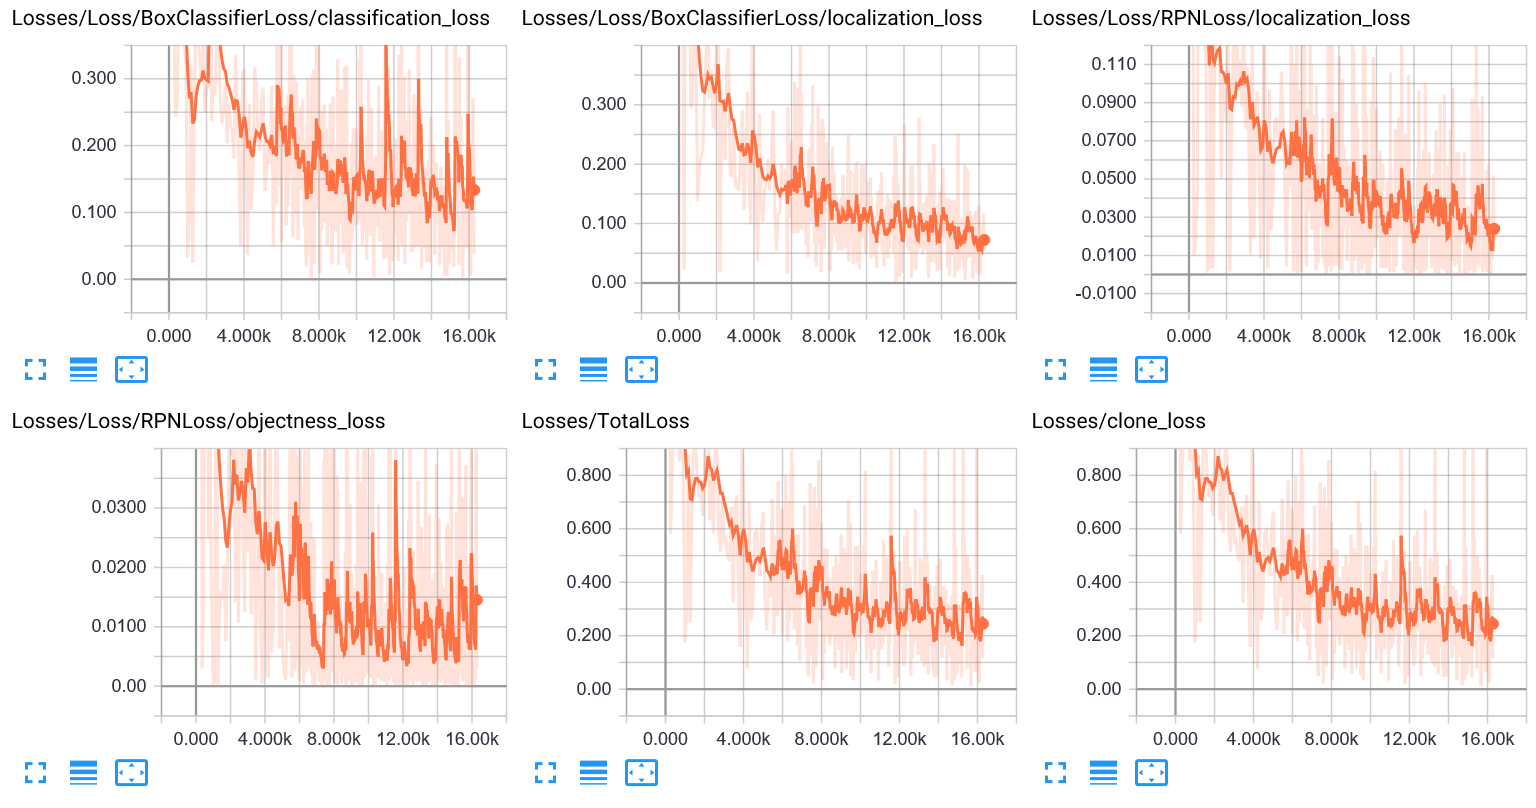
\includegraphics[width=15cm]{img/tests/tensorflow_pklot_full_train.png}
    \centering
    \caption{Entrainement sur le corpus \textit{PKLot} (graphes par \textit{Tensorboard})}
    \label{fig:tensorflow_train}
\end{figure} 

On distingue plusieurs fonctions objectifs:
\begin{description}
    \item[\textit{Classification loss}] La perte au fil des itérations lors de la classification. 
    \item[\textit{Localization loss}] Présente à quel point les \textit{bounding box} désignant les voitures sont bien localisées.
    \item[\textit{Objectness loss}] Pour chaque \textit{bounding box}, il s'agit de définir si c'est une voiture ou l'arrière-plan
    \item[\textit{Total loss}] Présente une combinaison des toutes les fonctions de pertes.
\end{description}

L'entrainement a été stoppé après 16000 itérations (plus de 2 jours de calculs). En effet, il semble qu'un certain palier ai été atteint. Aussi, plus d'itérations pourraient entrainer à un sur-apprentissage. Les nombres d'itérations 4000 et 16000 ont été évalués, ainsi que le modèle pré-entrainé.

Afin d'effectuer les tests, il est nécessaire de choisir un score minimum. Celui-ci indique, pour chaque objet détecté, à quel point l'algorithme est confiant sur sa prédiction. La figure \ref{fig:tensorflow_bb} présente une détection effectuée sur une image du \textit{dataset} \textit{PKLot}. 

\begin{figure}[ht]
    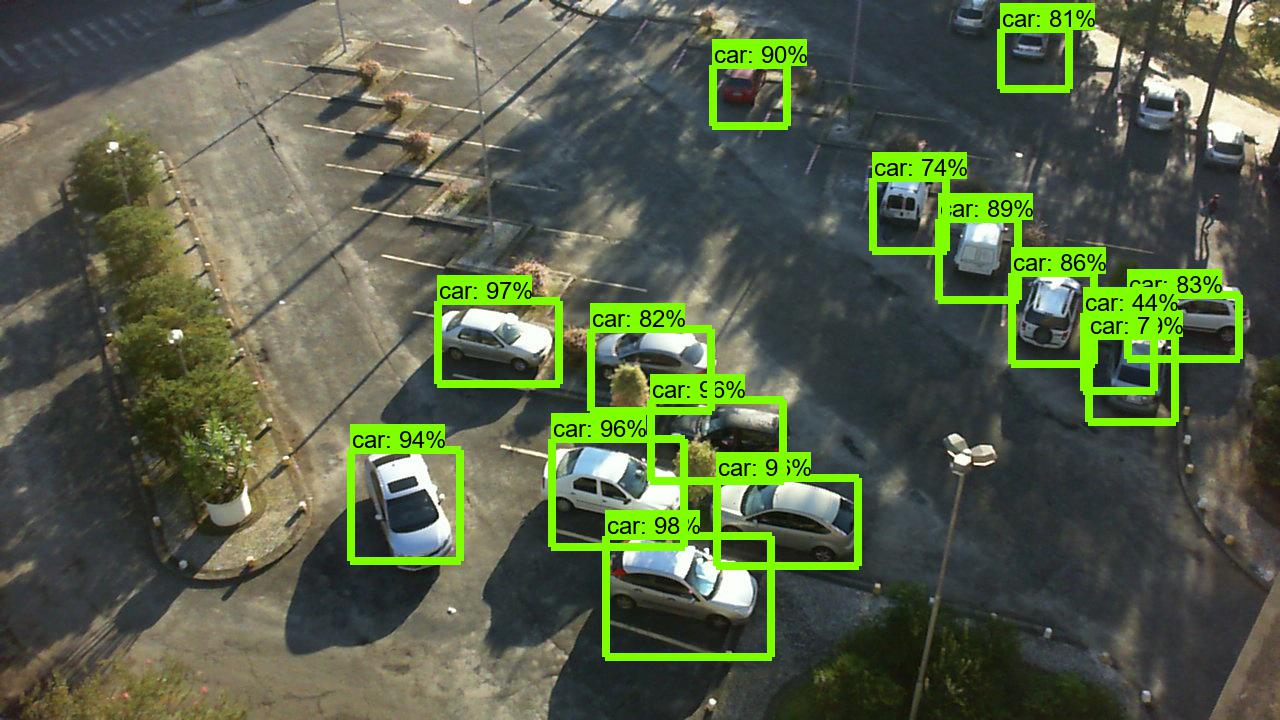
\includegraphics[width=10cm]{img/tests/tensorflow_bb.jpg}
    \centering
    \caption{Exemple de détection sur un entrainement de 4000 itérations}
    \label{fig:tensorflow_bb}
\end{figure} 

Les scores sont généralement supérieurs à 75\%. Il est possible de remarquer un faux positif d'un score de 44\%. Un seuil de 70\% a été défini, afin d'obtenir une certaine marge, et réduire le nombre de faux positif. Cependant, il faut remarquer que si le modèle \textit{Faster RCNN} est utilisé, ce seuil à du être abaissé à 20\% pour obtenir des résultats raisonnables. Ceci permet aussi d'indiquer que l'utilisation d'un modèle non ré-entrainé ne permet pas une grande confiance en l'algorithme.

\paragraph{Résultats}

Le tableau \ref{tab:rcnn_results} présente les résultats du modèles \textit{Faster RCNN} pré-entrainé (0 itérations), ainsi qu'entrainé avec 4000 et 1600 itérations supplémentaires sur le corpus d'images \textit{PKLot}. Les calculs qui ont été effectués ont été décrit en section \ref{conception.eval} \itnameref{conception.eval}.

\paragraph{\textit{Cars dataset}}

Un entrainement sur le \textit{dataset} \textit{Cars}, vu en section \ref{conception.dataset} \itnameref{conception.dataset}, a aussi été testé. Cependant, les résultats obtenus n'étaient pas bons, où un entrainement entrainait des résultats moins bon que le modèle pré-entrainé. Il est possible que ce corpus ne soit pas adapté pour des images de parkings, car les angles de vues prise des voitures et leurs tailles n'est pas similaire. Il n'a donc pas été souhaité de préciser les détails des résultats ici.

\begin{table}[ht]
\centering
\begin{tabular}{@{}ll@{}}
\toprule
N° itération & RMSE \\ \midrule
$0$            & $32.06564071$ \\
$4000$         & $10.4427355$ \\
$16000$        & $22.88589282$ \\ \bottomrule
\end{tabular}
\caption{\textit{Faster RCNN} - Résultats}
\label{tab:rcnn_results}
\end{table}

Le modèle entrainé 4000 fois semble le meilleur lors de l'évaluation. La cause est sans doute un sur-entrainement du modèle à 16000 itérations, ce qui ne permet pas de le généraliser suffisamment.

\todo{Graphiques ? Parler genre qu'avec les caméras où ya beaucoup de voiture, ça marche moins bien}

\section{Yolo v3}

Le modèle \textit{Yolo} a aussi été évalué. Un modèle pré-entrainé sur le corpus d'images \textit{Coco}\autocite{data:coco} à été utilisé.

\begin{figure}[ht]
    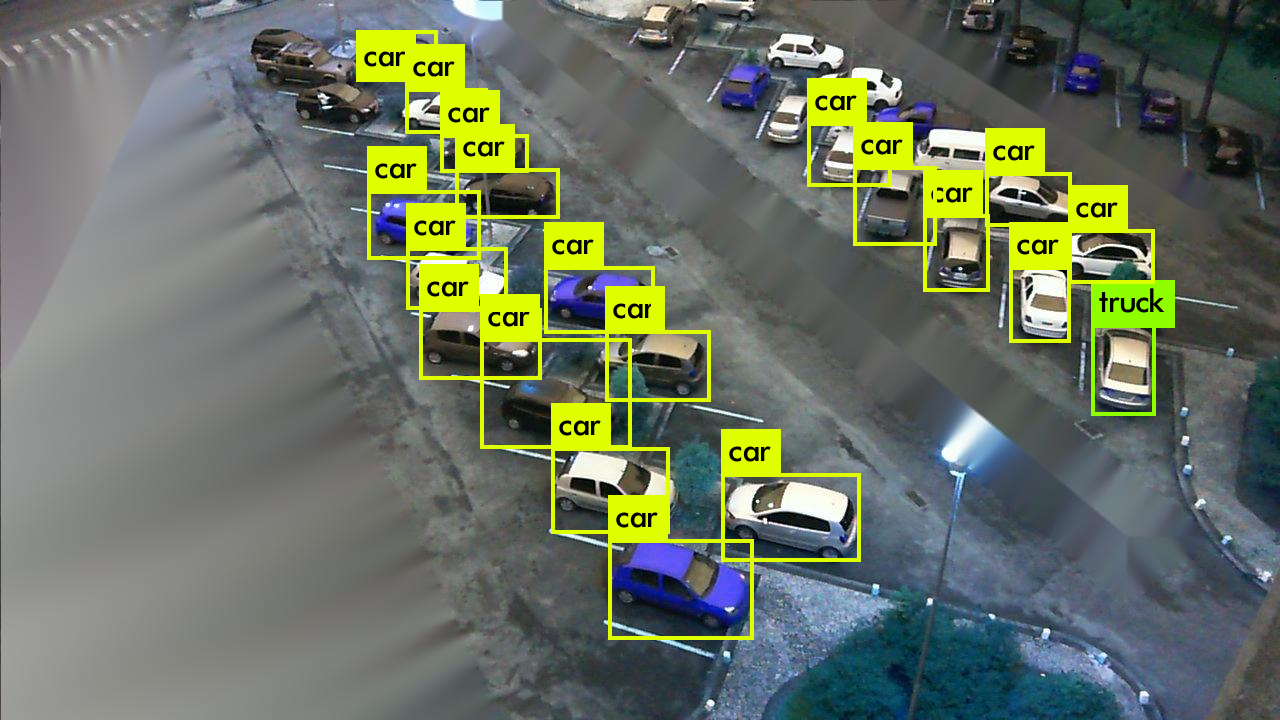
\includegraphics[width=10cm]{img/tests/yolo_bb.png}
    \centering
    \caption{Exemple de détection avec un modèle \textit{Yolo v3} pré-entrainé sur \textit{Coco}}
    \label{fig:yolo_bb}
\end{figure} 

Le réseau de neurones a aussi été entrainé sur le \textit{dataset} \textit{PKLot}, jusqu'à un nombre de 200 itérations. Cependant, les résultats n'ont pas été concluants, où que peu de voitures ont pu être détectées. 200 itérations semble un nombre très faible. Cependant, le temps d'entrainement nécessaires était trop grand, où moins de 100 itérations par jours étaient effectuées. Ainsi ici, aux vues des résultats médiocres, il n'a pas été souhaités de les intégrer à cette évaluations. Ainsi, seul le modèle pré-entrainé sur le corpus d'images \textit{Coco} a été effectué. 

De la même manière qu'auparavant, l'erreur au carré moyenne a été calculée sur le nombre de voiture détectées. On en trouvera le résultat en figure \ref{tab:yolo_results}.

\begin{table}[ht]
\centering
\begin{tabular}{@{}ll@{}}
\toprule
Modèle & RMSE \\ \midrule
Yolo v3 entrainé sur \textit{Coco}  & $34.75053725$ \\ \bottomrule
\end{tabular}
\caption{\textit{Yolo} - Résultats}
\label{tab:yolo_results}
\end{table}

\section{Choix final} \label{tests.final}

A la vues des résultats précédent, il semble que le meilleur algorithme soit le modèle \textit{Faster RCNN} ré-entrainé sur \textit{PKLot} avec 4000 itérations supplémentaires. Il faut noter que ces résultats ont été obtenus à l'aide du corpus d'images \textit{PKLot}: ainsi, certains paramètres, comme le seuil de détection, doit peut-être être modifié. 


\section{Tests en conditions réels}
parler vite fait des résultats sur la caméra